\chapter{Communication and Measurement System}
In order to analyse the different receiver designs described in
\chapref{chap:rx} and to experiment with different channels
and system parameters a versatile comminication system
including a simulation framework and interfaces to the hardware
was needed. \\

The primary aim of the setup is to show, that multi-gigabit per second
throughput is possible using high modulation and wide channels.
Also the effect of phase noise and other performance limiting impairments
were investigated. \\

To achiev all this goals a flexible Matlab script supporting
many different configurations was written. It is able to simulate
the different receivers designs but also interfaces to the hardware
to replace the \gls{RF} parts by real hardware. Matlab was chosen
because of it's widespread use in communication systems research. \\

To optimally contribute to existing work, many parameters including
the important parts of the frame structure as well as modulation
schemes were done according to the proposed IEEE 802.11ad standard.
Since this system is soley for research and to avoid spending any
time on unnecessary features, the used system is not compliant to the
proposed standard though. \\

In all our experiments only one sender and one receiver is used.
Therefor there is no need for and frequency and time slot acquisition
method. During each run of the simulation script, exactly one frame
of a fixed size is transmitted and received.
When the hardware is used, the waveform of this frame is loaded into
the \gls{AWG} and retransmitted is an loop.
The acquisition hardware uses a trigger signal generated by the \gls{AWG}
to always start shortely before the frame starts.

\section{Frame structure}
\label{sec:sys_frame_struct}
The basic idea of a frame in a system like the one proposed by
IEEE 802.11ad is to form one chunk of data which is transmitted without
and interruption and allows the receiver to recover as much data as
possible. \\
There is no context except fixed parameters stored accross consecutive
frames. Therefor all needed parameters like frequency offset, channel
response, phase corrections etc. are estimated on a per frame basis. \\

Most parameters like frequency offset, channel response, and
synchronization in time can be done only once on the beginning of the
frame using a fixed preamble.
The channel response is than assumed to be constant enough during
the whole frame such that last data symbol of the frame can still be
recoverd by the receiver. This assumption limits the maximum length a frame
can have. \\

The length of this preamble mainly depends on the maximal delay spread
\footnote{The difference in time of the arrival of the earlist and the
  latest significant energy component devided by the symbol length
  $T_s = \frac{1}{f_s}$} and the precision of the used oscillators defining
the maximal frequency offset. \\

The absolut phase of the first data symbol is detected and corrected by the
channel correction. Is our case of a system working on 60 GHz, the
phase is havely affected by phase noise as it was characterized in
\todo{cite radoslav's work}. This results in consecutive symbols to be
rotated such that less than hundred symbols at $f_s = 1.8 \text{GHz}$
could be transmitted before the rotation is so severe that detection
becomes impossible. \\

Because only a frew 100 data symbols per frame would mean,
that a significant part of transmission time and energy is spent
of the preamble overhead, the data is split into data blocks each having
it's own phase noise estimation. \\

The used frame structure is shown in \figref{fig:sys_frame_struct}.
The \gls{FES} field is described in \secref{sec:sys_fes},
the \gls{CES} field in \secref{sec:sys_ces},
the Data fields in \secref{sec:sys_data} and the
\gls{PES} field in \secref{sec:sys_pes}.

\begin{figure}[ht]
  \centering
  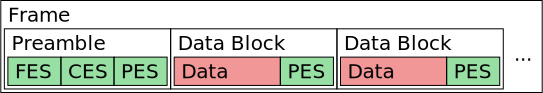
\includegraphics[width=0.7\textwidth]{figures/frame_struct}
  \caption{Frame Structure}
  \label{fig:sys_frame_struct}
\end{figure}

\section{Modulation and Pulse Shaping Scheme}
A constant symbol rate $f_s$ was used in for the whole frame. \\

For the data fields \gls{BPSK}, \gls{QPSK} and arbitrary, even
\gls{QAM} modulations were implemented. Therby the datarate
can be maximized depending on the \gls{SNR}. \\

Because the training and estimation fields are not used to
transmitt any information but only to synchronize in time
and frequency and to measure channel properties they were all
modulated using \gls{BPSK}. \\

A \gls{RRC}-filter was used for pulse shaping. It has the big advantage that
the same filter can be used for transmission and reception. \\

\section{Frequency Offset Estimation and Correction}
The \gls{FES} field is used to do a simple, non standard complient frequency
offset estimation. It consists of $L$ copies of the same random data block $d$
of length $l$.
The frequency offset is than estimated by calculating the average phase
difference $a$ of each block $k$ with block the previous block $k - 1$
\eqref{eq:sys_foffset_a}. The frequency offset estimation
$f_{\text{offset est.}}$ can than be calculated using \eqref{eq:sys_foffset}
where $f_s$ is the sample rate. \\

\begin{subequations}
  \begin{alignat}{2}
    a &= \frac{1}{(L-1) * l}
    \sum_{i=1}^{L-1} \sum_{j=0}^{l-1} \bar{d[i][k-1]} \cdot d[i][k]
    \label{eq:sys_foffset_a} \\
    f_{\text{offset est.}} &= \frac{a}{2 \pi} * \frac{f_s}{l}
    \label{eq:sys_foffset}
  \end{alignat}
\end{subequations}

\section{Time Synchronization \& Channel Estimation and Correction}
\todo{add time sync explanation}
The \gls{CES} field consists of Golay complementary sequences which
have very specific autocorrelation properties as described in
\todo{cite goaly paper} and can be used to build an very elegant
channel estimator as described in \todo{cite to goaly estimation paper}. \\

In our case a total of $2 \cdot 512 + 128 = 1152$ symbols plus
a cyclic prefix of $128$ symbols are used resulting in a \gls{CES} field
length of 1280.

\section{Data Blocks and Data Fields}
As described earlier, the data is split up in multiple data blocks
each having it's own \gls{PES} field after the data block.
Together with the \gls{PES} field at the end of the preamble, this forms
a cyclic structure which allows each data block to be transformed
from time to frequency domain by an \gls{FFT} and back to time domain
by an \gls{IFFT} without any error due to the block boundries.
This is very usefull when channel correction is performend in frequency domain.

\section{Phase Estimation and Correction}
The \gls{PES} field at the end of each data block is used to update
the current phase offset estimation which is than used for the correction
of the next data block. The field consists of a $l=64$ symbol long Golay
sequence eventhough the estimation would also work on random data. \\

The phase noise correction works as follows. For each data block
the following steps are performed:

\begin{enumerate}
\item The \gls{PES} field of the current block is corrected
  using the newst $\varphi_{\text{offset est.}}$.
  The correction is a complex multiplication \eqref{eq:sys_pes_correct}
  where $s[i] = p[i]$ are the uncorrected and
  $s_{\text{corr}}[i] = p_{\text{corr}}[i]$ are the corrected \gls{PES} symbols.
  $\varphi_{\text{offset est.}}$ is zero for the first block.
\item The current \gls{PES} field $p_{\text{corr}}[i]$
  is correlated with the first \gls{PES} field $p_{\text{first}}$
  to get the mean angle $m$ \eqref{eq:sys_pes_angle}.
\item The phase estimation is updated:
  $\varphi_{\text{offset est.}} := \varphi_{\text{offset est.}} + m$
\item The current data block is corrected using \eqref{eq:sys_pes_correct}
  where $s[i] = d[i]$ are the uncorrected and
  $s_{\text{corr}}[i] = d_{\text{corr}}[i]$ are the corrected data symbols.
\end{enumerate}

\begin{align}
  \label{eq:sys_pes_correct}
  s_{\text{corr}}[i] = s[i] \cdot \exp(-j \cdot \varphi_{\text{offset est.}})
  \;\;\; \forall i \in {0, 1, \dots, l-1}
\end{align}

\begin{align}
  \label{eq:sys_pes_angle}
  m = \frac{1}{l}
  \sum_{i=0}^{l-1} \angle(p_{\text{corr}}[i] \cdot p_{\text{first}}[i])
\end{align}
